\section{Starting a New Project}


To start working on a new design we first have to define a new 
{\it design project}.
Quartus Prime software makes the designer's task easy by providing support in the form
of a {\it wizard}.
Create a new project as follows:
\begin{enumerate}
\item Select {\sf File $>$ New Project Wizard} and click {\sf Next} to 
reach the window in Figure~\ref{fig:4},
which asks for the name and directory of the project.

\item Set the working directory to be {\it introtutorial};
of course, you can use some other directory name of your choice if you prefer.
The project must have a name, which is usually the same as the 
top-level design entity that will be included in the project.
Choose {\it light} as the name for both the project
and the top-level entity, as shown in Figure~\ref{fig:4}.  Press {\sf Next}. 
Since we have not yet created the directory {\it introtutorial},
Quartus Prime software displays the pop-up box in Figure~\ref{fig:5} asking if it should create
the desired directory. Click {\sf Yes}, which leads to
the window in Figure~\ref{fig:5_1}.

\begin{figure}[H]
   \begin{center}
      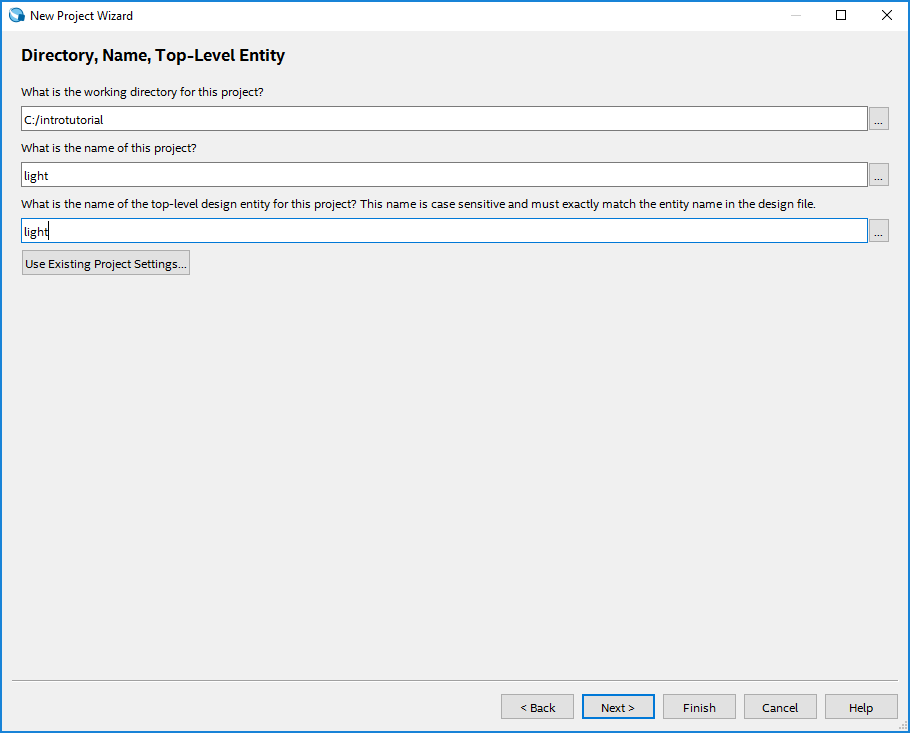
\includegraphics[scale=0.55]{figures/figure4.png}
   \caption{Creation of a new project.}
	 \label{fig:4}
	 \end{center}
\end{figure}

\begin{figure}[H]
   \begin{center}
      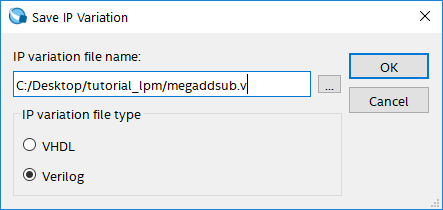
\includegraphics[scale=0.55]{figures/figure5.png}
   \caption{Quartus Prime software can create a new directory for the project.} 
	 \label{fig:5}
	 \end{center}
\end{figure}

\begin{figure}[H]
   \begin{center}
      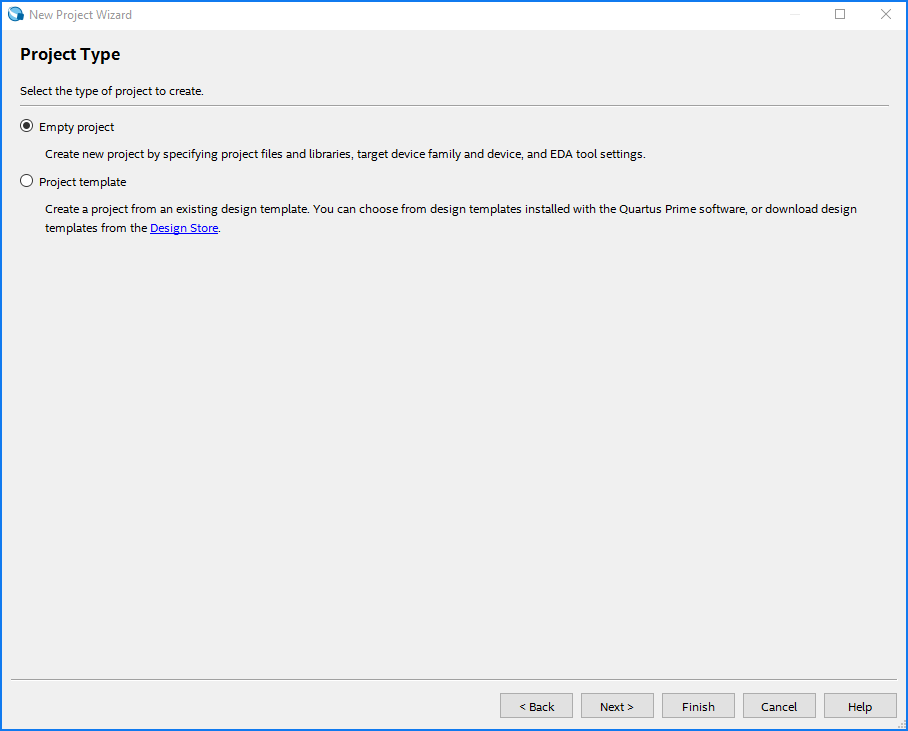
\includegraphics[scale=0.55]{figures/figure5_1.png}
   \caption{Choosing the project type.} 
	 \label{fig:5_1}
	 \end{center}
\end{figure}

\item The {\sf Project Type} window, shown in Figure~\ref{fig:5_1}, allows you to choose from
the {\sf Empty project} and the {\sf Project template} options. For this tutorial, choose {\sf Empty project} 
as we will be creating a project from scratch, and press {\sf Next} which leads to the window in Figure~\ref{fig:6}. 

\begin{figure}[H]
   \begin{center}
      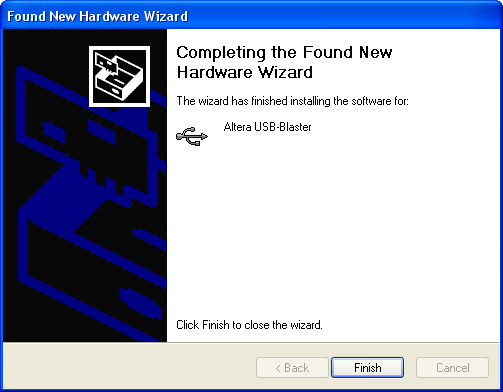
\includegraphics[scale=0.55]{figures/figure6.png}
   \caption{The wizard can include user-specified design files.} 
	 \label{fig:6}
	 \end{center}
\end{figure}

\item The wizard makes it easy to 
specify which existing files (if any) should be included in the project.
Assuming that we do not have any existing files, click {\sf Next}, which leads
to the window in Figure~\ref{fig:7}.

\begin{figure}[H]
   \begin{center}
      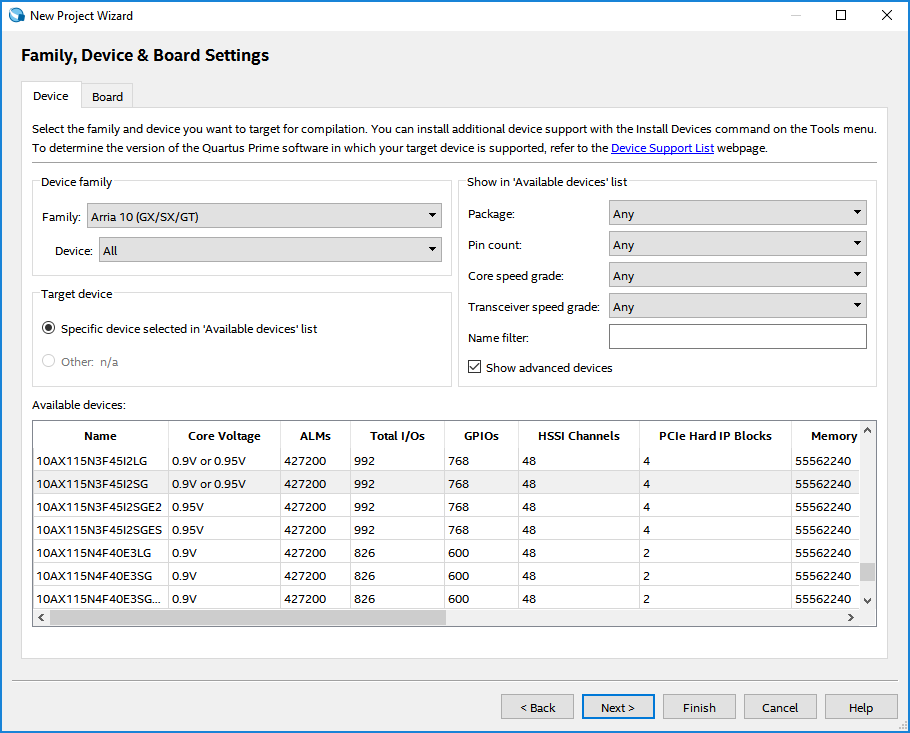
\includegraphics[scale=0.55]{figures/figure7.png}
   \caption{Choose the device family and a specific device.} 
	 \label{fig:7}
	 \end{center}
\end{figure}

\item We have to specify the type of device in which the designed circuit will 
be implemented.
Choose the Cyclone\textsuperscript{\textregistered} series device family for your DE-series board. 
We can let Quartus Prime software select a specific device in the family, 
or we can choose the device explicitly. 
We will take the latter approach. 
From the list of available devices, choose the appropriate device name for your DE-series board. A list of devices names on DE-series boards can be found in Table \ref{tab:device}. 
Press {\sf Next}, which opens the window in Figure~\ref{fig:8}.
 
\begin{table}[H]
	\begin{center}
	\begin{tabular}{| c | c |}
	\hline
	Board & Device Name \\
	\hline
	DE0-CV & Cyclone V 5CEBA4F23C7 \\
	\hline
	DE0-Nano & Cyclone IVE EP4CE22F17C6 \\
	\hline
	DE0-Nano-SoC & Cyclone V SoC 5CSEMA4U23C6\\
	\hline
	DE1-SoC & Cyclone V SoC 5CSEMA5F31C6 \\
	\hline
	DE2-115 & Cyclone IVE EP4CE115F29C7 \\
	\hline
	DE10-Lite & Max 10 10M50DAF484C7G \\
	\hline
	DE10-Standard & Cyclone V SoC 5CSXFC6D6F31C6 \\
	\hline
	DE10-Nano & Cyclone V SE 5CSEBA6U2317 \\
	\hline
	\end{tabular}
	\caption{DE-series FPGA device names}
	\label{tab:device}
	\end{center}
\end{table}

\begin{figure}[H]
   \begin{center}
      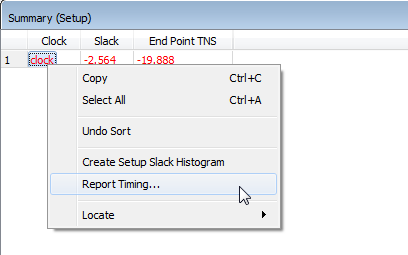
\includegraphics[scale=0.6]{figures/figure8.png}
   \caption{Other EDA tools can be specified.} 
	 \label{fig:8}
	 \end{center}
\end{figure}

\item The user can specify any third-party tools that should be used.
A commonly used term for CAD software for electronic circuits
is {\it EDA tools}, where the acronym stands for Electronic Design Automation.
This term is used in Quartus Prime messages that refer to third-party tools, 
which are the tools developed and marketed by companies other than Intel.
Since we will rely solely on Quartus Prime tools, we will not choose 
any other tools.  Press {\sf Next}.
 
\item A summary of the chosen settings appears in the screen shown in Figure~\ref{fig:9}.
Press {\sf Finish}, which returns to the main Quartus Prime window, 
but with {\it light} specified as the new project,
in the title bar, as indicated in Figure~\ref{fig:10}.
\end{enumerate}

\begin{figure}[H]
   \begin{center}
      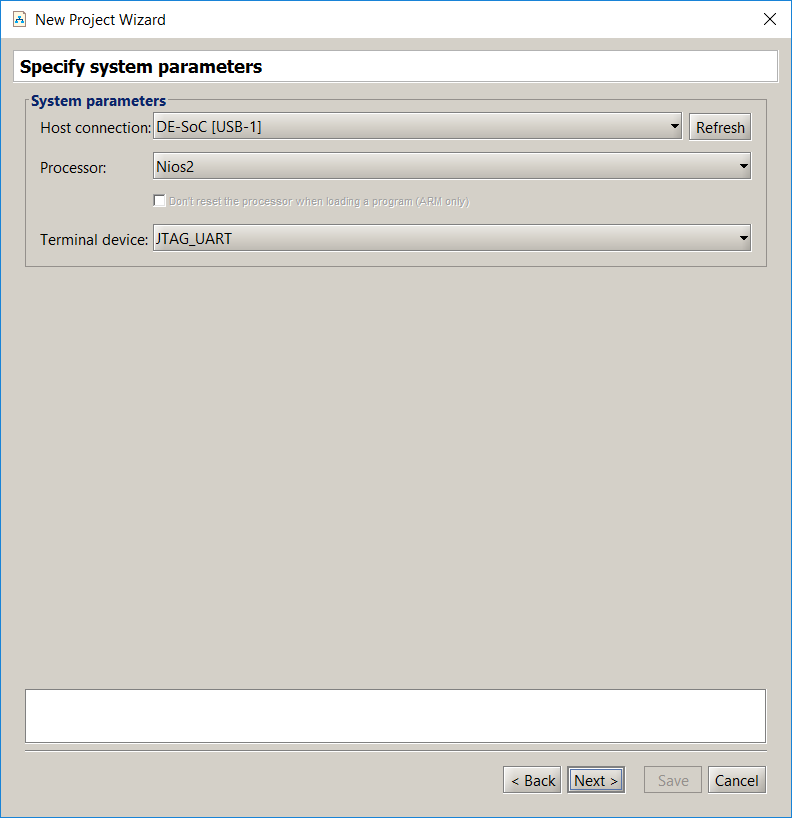
\includegraphics[scale=0.5]{figures/figure9.png}
   \caption{Summary of project settings.} 
	 \label{fig:9}
	 \end{center}
\end{figure}

\begin{figure}[H]
   \begin{center}
      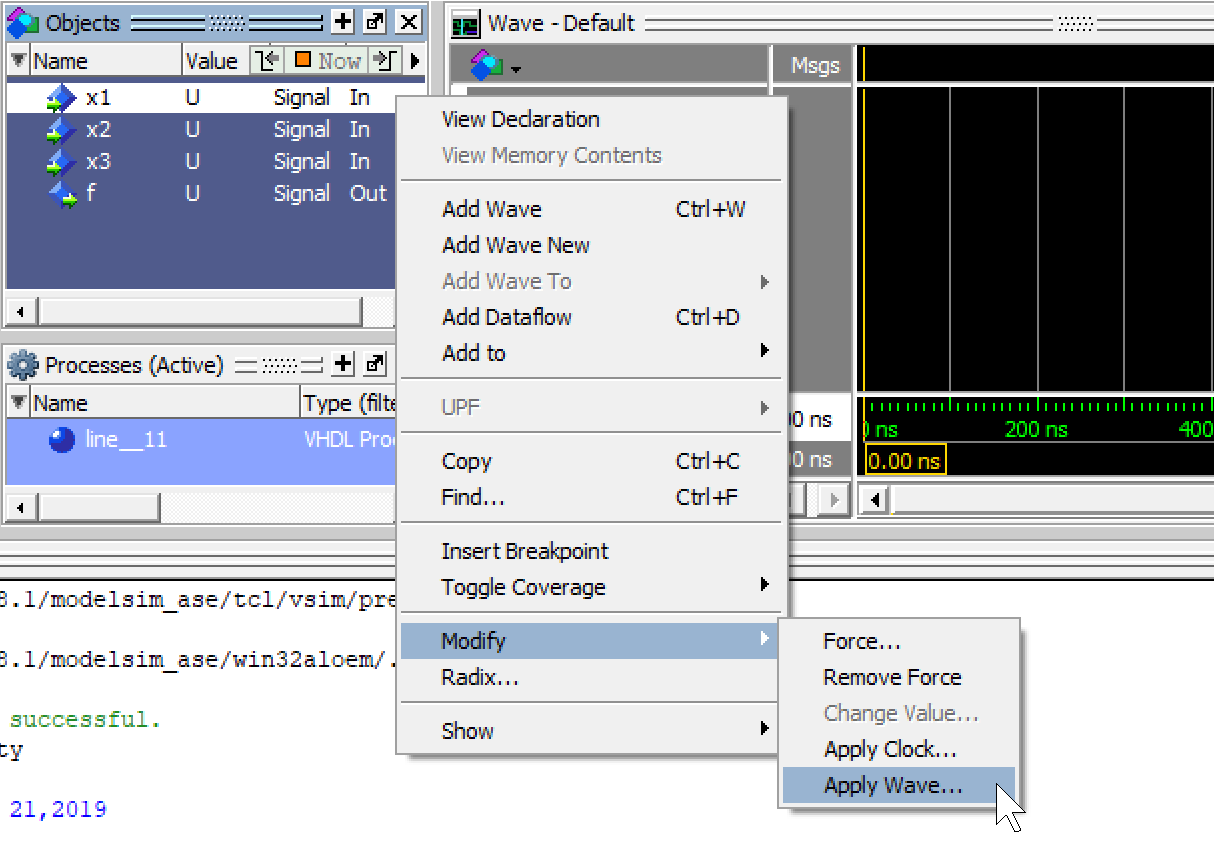
\includegraphics[scale=0.4]{figures/figure10.png}
   \caption{The Quartus Prime window for a created project.} 
	 \label{fig:10}
	 \end{center}
\end{figure}
